\documentclass[main]{subfiles}

\begin{document}
\section{ネットワーク設計}
図\ref{fig:inamura2}は本システム全体のネットワーク構成を表したものである。本システムはホテル内ネットワークでのみ使用することができる。なお,本システムはホテル内ネットワークでのみの使用を想定しており,インターネットからの接続は行わない.

サーバにはセキュリティ面を考慮し,ホテル内にサーバを設置する.従業員は,端末で無線通信によりホテル内ネットワークに接続し,HTTP通信によって本システムを使用する.本システムで予約情報を参照するために,データベースサーバに情報を要求する.

本開発では,ホテルと同様の環境での開発が出来ないため,クラウドサーバであるAmazon Web Services(AWS)を使用します.

\begin{figure}[H]
\begin{center}
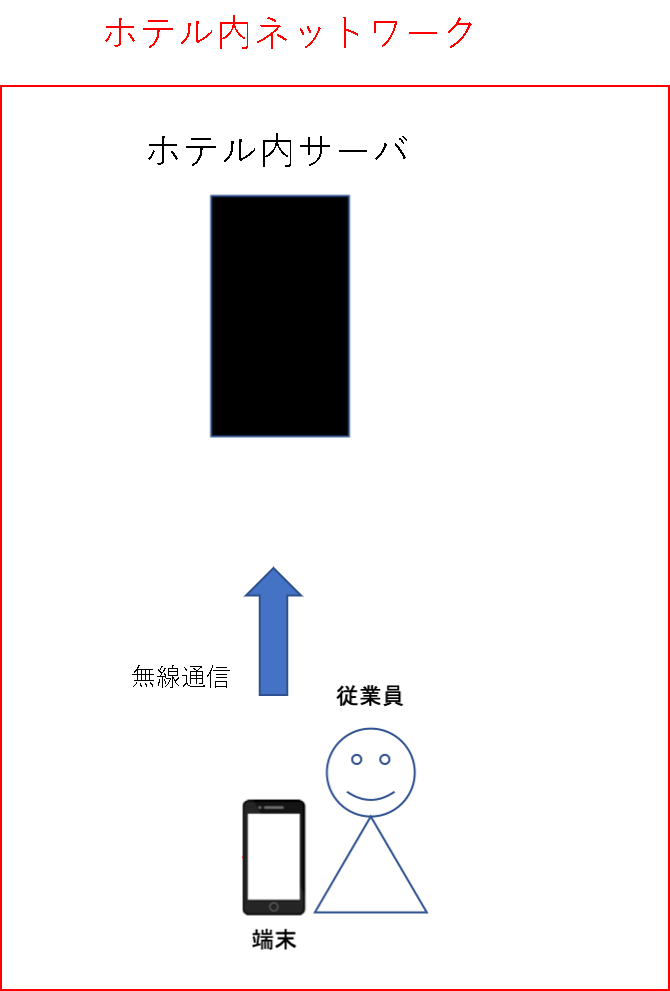
\includegraphics[scale=0.6]{kadai2-inamura3.png}
\caption{ネットワーク構成}
\label{fig:inamura2}
\end{center}
\end{figure}


\end{document}
